\documentclass[10pt]{article}
\usepackage[utf8]{inputenc}
\usepackage[T1]{fontenc}
\usepackage{amsmath}
\usepackage{amsfonts}
\usepackage{amssymb}
\usepackage[version=4]{mhchem}
\usepackage{stmaryrd}
\usepackage{graphicx}
\usepackage[export]{adjustbox}
\graphicspath{ {./images/} }
\usepackage{bbold}

\begin{document}
\section*{MATHEMATICS}
\section*{SECTION-A}
\begin{enumerate}
  \setcounter{enumi}{60}
  \item Consider the following statements:
\end{enumerate}

P : I have fever\\
Q : I will not take medicine\\
R : I will take rest\\
The statement "If I have fever, then I will take medicine and I will take rest" is equivalent to:\\
(1) \(((\sim \mathrm{P}) \vee \sim \mathrm{Q}) \wedge((\sim \mathrm{P}) \vee \mathrm{R})\)\\
(2) \(((\sim \mathrm{P}) \vee \sim \mathrm{Q}) \wedge((\sim \mathrm{P}) \vee \sim \mathrm{R})\)\\
(3) \((\mathrm{P} \vee \mathrm{Q}) \wedge((\sim \mathrm{P}) \vee \mathrm{R})\)\\
(4) \((\mathrm{P} \vee \sim \mathrm{Q}) \wedge(\mathrm{P} \vee \sim \mathrm{R})\)

\section*{Official Ans. by NTA (1)}
Allen Ans. (1)\\
Sol. \(\quad \mathrm{P} \rightarrow(\sim \mathrm{Q} \wedge \mathrm{R})\)\\
\(\sim P \vee(\sim Q \wedge R)\)\\
\((\sim \mathrm{P} \vee \sim \mathrm{Q}) \wedge(\sim \mathrm{P} \vee \mathrm{R})\)\\
62. Let A be a point on the x -axis. Common tangents are drawn from A to the curves \(\mathrm{x}^{2}+\mathrm{y}^{2}=8\) and \(\mathrm{y}^{2}=\) 16x. If one of these tangents touches the two curves at Q and R , then \((\mathrm{QR})^{2}\) is equal to\\
(1) 64\\
(2) 76\\
(3) 81\\
(4) 72

Official Ans. by NTA (4)\\
Allen Ans. (4)\\
Sol. \(y=m x+\frac{4}{m}\)\\
\(\frac{\left|\frac{4}{\mathrm{~m}}\right|}{\sqrt{1+\mathrm{m}^{2}}}=2 \sqrt{2} \therefore \mathrm{~m}= \pm 1\)\\
\(\mathrm{y}= \pm \mathrm{x} \pm 4\). Point of contact on parabola\\
Let \(\mathrm{m}=1,\left(\frac{\mathrm{a}}{\mathrm{m}^{2}}, \frac{2 \mathrm{a}}{\mathrm{m}}\right)\)\\
R \((4,8)\)\\
Point of contact on circle Q ( \(-2,2\) )\\
\(\therefore(\mathrm{QR})^{2}=36+36=72\)

\section*{TEST PAPER WITH SOLUTION}
\begin{enumerate}
  \setcounter{enumi}{62}
  \item Let \(q\) be the maximum integral value of \(p\) in \([0,10]\) for which the roots of the equation \(x^{2}-p x+\frac{5}{4} p=0\) are rational. Then the area of the region \(\{(\mathrm{x}, \mathrm{y}): 0 \leq \mathrm{y} \left.\leq(\mathrm{x}-\mathrm{q})^{2}, 0 \leq \mathrm{x} \leq \mathrm{q}\right\}\) is\\
(1) 243\\
(2) 25\\
(3) \(\frac{125}{3}\)\\
(4) 164
\end{enumerate}

Official Ans. by NTA (1)\\
Allen Ans. (1)\\
Sol. \(\quad \mathrm{x}^{2}-\mathrm{px}+\frac{5 \mathrm{p}}{4}=0\)\\
\(\mathrm{D}=\mathrm{p}^{2}-5 \mathrm{p}=\mathrm{p}(\mathrm{p}-5)\)\\
\(\therefore \mathrm{q}=9\)\\
\(0 \leq \mathrm{y} \leq(\mathrm{x}-9)^{2}\)\\
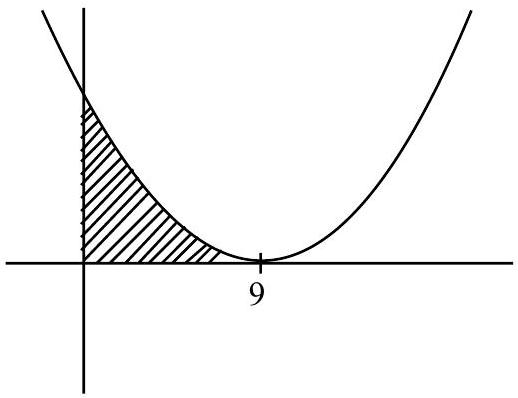
\includegraphics[max width=\textwidth, center]{2025_10_03_ad9ac098ef72e20a69f1g-1}

Area \(=\int_{0}^{9}(x-9)^{2} d x=243\)\\
64. If the functions \(f(x)=\frac{x^{3}}{3}+2 b x+\frac{a x^{2}}{2}\) and \(g(x)=\frac{x^{3}}{3}+a x+b x^{2}, a \neq 2 b\) have a common extreme point, then \(\mathrm{a}+2 \mathrm{~b}+7\) is equal to\\
(1) 4\\
(2) \(\frac{3}{2}\)\\
(3) 3\\
(4) 6

Official Ans. by NTA (4)\\
Allen Ans. (4)

Sol. \(f^{\prime}(x)=x^{2}+2 b+a x\)\\
\(\mathrm{g}^{\prime}(\mathrm{x})=\mathrm{x}^{2}+\mathrm{a}+2 \mathrm{bx}\)\\
\((2 b-a)-x(2 b-a)=0\)\\
\(\therefore \mathrm{x}=1\) is the common root\\
Put \(\mathrm{x}=1\) in \(\mathrm{f}^{\prime}(\mathrm{x})=0\) or \(\mathrm{g}^{\prime}(\mathrm{x})=0\)\\
\(1+2 b+a=0\)\\
\(7+2 b+a=6\)\\
65. The range of the function \(f(x)=\sqrt{3-x}+\sqrt{2+x}\) is\\
(1) \([\sqrt{5}, \sqrt{10}]\)\\
(2) \([2 \sqrt{2}, \sqrt{11}]\)\\
(3) \([\sqrt{5}, \sqrt{13}]\)\\
(4) \([\sqrt{2}, \sqrt{7}]\)

Official Ans. by NTA (1)\\
Allen Ans. (1)\\
Sol. \(\quad y^{2}=3-x+2+x+2 \sqrt{(3-x)(2+x)}\)\\
\(=5+2 \sqrt{6+x-x^{2}}\)\\
\(\mathrm{y}^{2}=5+2 \sqrt{\frac{25}{4}-\left(\mathrm{x}-\frac{1}{2}\right)^{2}}\)\\
\(\mathrm{y}_{\text {max }}=\sqrt{5+5}=\sqrt{10}\)\\
\(\mathrm{y}_{\text {min }}=\sqrt{5}\)\\
66. The solution of the differential equation\\
\(\frac{d y}{d x}=-\left(\frac{x^{2}+3 y^{2}}{3 x^{2}+y^{2}}\right), y(1)=0\) is\\
(1) \(\log _{\mathrm{e}}|\mathrm{x}+\mathrm{y}|-\frac{\mathrm{xy}}{(\mathrm{x}+\mathrm{y})^{2}}=0\)\\
(2) \(\log _{\mathrm{e}}|\mathrm{x}+\mathrm{y}|+\frac{\mathrm{xy}}{(\mathrm{x}+\mathrm{y})^{2}}=0\)\\
(3) \(\log _{e}|x+y|+\frac{2 x y}{(x+y)^{2}}=0\)\\
(4) \(\log _{\mathrm{e}}|\mathrm{x}+\mathrm{y}|-\frac{2 \mathrm{xy}}{(\mathrm{x}+\mathrm{y})^{2}}=0\)

Official Ans. by NTA (3)\\
Allen Ans. (3)

Sol. Put y = vx\\
\(v+x \frac{d v}{d x}=-\left(\frac{1+3 v^{2}}{3+v^{2}}\right)\)\\
\(x \frac{d v}{d x}=-\frac{(v+1)^{3}}{3+v^{2}}\)\\
\(\frac{\left(3+v^{2}\right) d v}{(v+1)^{3}}+\frac{d x}{x}=0\)\\
\(\int \frac{4 d v}{(v+1)^{3}}+\int \frac{d v}{v+1}-\int \frac{2 d v}{(v+1)^{2}}+\int \frac{d x}{x}=0\)\\
\(\frac{-2}{(\mathrm{v}+1)^{2}}+\ln (\mathrm{v}+1)+\frac{2}{\mathrm{v}+1}+\ln \mathrm{x}=\mathrm{c}\)\\
\(\frac{-2 x^{2}}{(x+y)^{2}}+\ln \left(\frac{x+y}{x}\right)+\frac{2 x}{x+y}+\ln x=c\)\\
\(\frac{2 x y}{(x+y)^{2}}+\ln (x+y)=c\)\\
\(\therefore \mathrm{c}=0\), as \(\mathrm{x}=1, \mathrm{y}=0\)\\
\(\therefore \frac{2 x y}{(x+y)^{2}}+\ln (x+y)=0\)\\
67. Let \(x=(8 \sqrt{3}+13)^{13}\) and \(y=(7 \sqrt{2}+9)^{9}\). If [t] denotes the greatest integer \(\leq \mathrm{t}\), then\\
(1) \([x]+[y]\) is even\\
(2) \([x]\) is odd but \([y]\) is even\\
(3) \([x]\) is even but \([y]\) is odd\\
(4) \([x]\) and \([y]\) are both odd

Official Ans. by NTA (1)\\
Allen Ans. (1)\\
Sol. \(\mathrm{x}=(8 \sqrt{3}+13)={ }^{13} \mathrm{C}_{0} \cdot(8 \sqrt{3})^{13}+{ }^{13} \mathrm{C}_{1}(8 \sqrt{3})^{12}(13)^{1}+\ldots\)\\
\(x^{\prime}=(8 \sqrt{3}-13)^{13}={ }^{13} C_{0}(8 \sqrt{3})^{13}-{ }^{13} C_{1}(8 \sqrt{3})^{12}(13)^{1}+\ldots\)\\
\(x-x^{\prime}=2\left[{ }^{13} C_{1} \cdot(8 \sqrt{3})^{12}(13)^{1}+{ }^{13} C_{3}(8 \sqrt{3})^{10} \cdot(13)^{3} \cdots\right]\)\\
therefore, \(\mathrm{x}-\mathrm{x}^{\prime}\) is even integer, hence \([\mathrm{x}]\) is even\\
Now, \(\mathrm{y}=(7 \sqrt{2}+9)^{9}={ }^{9} \mathrm{C}_{0}(7 \sqrt{2})^{9}+{ }^{9} \mathrm{C}_{1}(7 \sqrt{2})^{8}(9)^{1}\)\\
\(+{ }^{9} \mathrm{C}_{2}(7 \sqrt{2})^{7}(9)^{2} \ldots \ldots\)\\
\(\mathrm{y}^{\prime}=(7 \sqrt{2}-9)^{9}={ }^{9} \mathrm{C}_{0}(7 \sqrt{2})^{9}-{ }^{9} \mathrm{C}_{1}(7 \sqrt{2})^{8}(9)^{1}\)\\
\(+{ }^{9} \mathrm{C}_{2}(7 \sqrt{2})^{7}(9)^{2} \ldots \ldots\)\\
\(y-y^{\prime}=2\left[{ }^{9} C_{1}(7 \sqrt{2})^{8}(9)^{1}+{ }^{9} C_{3}(7 \sqrt{2})^{6}(9)^{3}+\ldots\right]\)\\
\(y-y^{\prime}=\) Even integer, hence \([y]\) is even\\
68. A vector \(\overrightarrow{\mathrm{v}}\) in the first octant is inclined to the \(\mathrm{x}-\) axis at \(60^{\circ}\), to the \(y\)-axis at \(45^{\circ}\) and to the z-axis at an acute angle. If a plane passing through the points \((\sqrt{2},-1,1)\) and \((\mathrm{a}, \mathrm{b}, \mathrm{c})\), is normal to \(\overrightarrow{\mathrm{v}}\), then\\
(1) \(\sqrt{2} a+b+c=1\)\\
(2) \(a+b+\sqrt{2} c=1\)\\
(3) \(a+\sqrt{2} b+c=1\)\\
(4) \(\sqrt{2} a-b+c=1\)

Official Ans. by NTA (3)\\
Allen Ans. (3)\\
Sol. \(\hat{v}=\cos 60^{\circ} \hat{i}+\cos 45^{\circ} \hat{j}+\cos \gamma \hat{k}\)\\
\(\Rightarrow \frac{1}{4}+\frac{1}{2}+\cos ^{2} \gamma=1 \quad(\gamma \rightarrow\) Acute \()\)\\
\(\Rightarrow \cos \gamma=\frac{1}{2}\)\\
\(\Rightarrow \gamma=60^{\circ}\)\\
Equation of plane is\\
\(\frac{1}{2}(x-\sqrt{2})+\frac{1}{\sqrt{2}}(y+1)+\frac{1}{2}(z-1)=0\)\\
\(\Rightarrow x+\sqrt{2} y+z=1\)\\
( \(\mathrm{a}, \mathrm{b}, \mathrm{c}\) ) lies on it.\\
\(\Rightarrow a+\sqrt{2} b+c=1\)\\
69. Let \(f, g\) and \(h\) be the real valued functions defined on \(\mathbb{R}\) as \(f(x)=\left\{\begin{array}{cc}\frac{x}{|x|}, & x \neq 0 \\ 1, & x=0\end{array}\right.\),\\
\(g(x)=\left\{\begin{array}{cl}\frac{\sin (x+1)}{(x+1)}, & x \neq-1 \\ 1, & x=-1\end{array}\right.\) and \(h(x)=2[x]-f(x)\), where \([\mathrm{x}]\) is the greatest integer \(\leq \mathrm{x}\). Then the value of \(\lim _{x \rightarrow 1} g(h(x-1))\) is\\
(1) 1\\
(2) \(\sin (1)\)\\
(3) -1\\
(4) 0

Official Ans. by NTA (1)\\
Allen Ans. (1)

Sol. \(\quad \mathrm{LHL}=\lim _{\mathrm{k} \rightarrow 0} \mathrm{~g}(\mathrm{~h}(-\mathrm{k})) \quad, \mathrm{k}>0\)\\
\(=\lim _{\mathrm{k} \rightarrow 0} \mathrm{~g}(-2+1) \quad \because \mathrm{f}(\mathrm{x})=-1 \forall \mathrm{x}<0\)\\
\(=\mathrm{g}(-1)=1\)\\
\(\mathrm{RHL}=\lim _{\mathrm{k} \rightarrow 0} \mathrm{~g}(\mathrm{~h}(\mathrm{k})) \quad, \mathrm{k}>0\)\\
\(=\lim _{\mathrm{k} \rightarrow 0} \mathrm{~g}(-1) \quad, \because \mathrm{f}(\mathrm{x})=1, \forall \mathrm{x}>0\)\\
\(=1\)\\
70. The number of ways of selecting two numbers \(a\) and \(b\), \(\mathrm{a} \in\{2,4,6, \ldots . ., 100\} \quad\) and \(\mathrm{b} \in\{1,3,5, \ldots . ., 99\}\) such that 2 is the remainder when \(\mathrm{a}+\mathrm{b}\) is divided by 23 is\\
(1) 186\\
(2) 54\\
(3) 108\\
(4) 268

Official Ans. by NTA (3)\\
Allen Ans. (3)\\
Sol. \(\mathrm{a} \in\{2,4,6,8,10, \ldots ., 100\}\)\\
\(\mathrm{b} \in\{1,3,5,7,9, \ldots . ., 99\}\)\\
Now, \(\mathrm{a}+\mathrm{b} \in\{25,71,117,163\}\)\\
(i) \(a+b=25\), no. of ordered pairs (a, b) is 12\\
(ii) \(a+b=71\), no. of ordered pairs ( \(a, b\) ) is 35\\
(iii) \(a+b=117\), no. of ordered pairs ( \(a, b\) ) is 42\\
(iv) \(a+b=163\), no. of ordered pairs ( \(a, b\) ) is 19\\
\(\therefore\) total \(=108\) pairs\\
71. If P is a \(3 \times 3\) real matrix such that \(\mathrm{P}^{\mathrm{T}}=\mathrm{aP}+(\mathrm{a}-1) \mathrm{I}\), where \(\mathrm{a}>1\), then\\
(1) P is a singular matrix\\
(2) \(|\operatorname{Adj} \mathrm{P}|>1\)\\
(3) \(|\operatorname{Adj} \mathrm{P}|=\frac{1}{2}\)\\
(4) \(|\operatorname{Adj} \mathrm{P}|=1\)

Official Ans. by NTA (4)\\
Allen Ans. (4)\\
Sol. \(\quad \mathrm{P}^{\mathrm{T}}=\mathrm{aP}+(\mathrm{a}-1) \mathrm{I}\)\\
\(\Rightarrow \mathrm{P}=\mathrm{aP}^{\mathrm{T}}+(\mathrm{a}-1) \mathrm{I}\)\\
\(\Rightarrow \mathrm{P}^{\mathrm{T}}-\mathrm{P}=\mathrm{a}\left(\mathrm{P}-\mathrm{P}^{\mathrm{T}}\right)\)\\
\(\Rightarrow \mathrm{P}=\mathrm{P}^{\mathrm{T}}\), as \(\mathrm{a} \neq-1\)\\
Now, \(\mathrm{P}=\mathrm{aP}+(\mathrm{a}-1) \mathrm{I}\)\\
\(\Rightarrow \mathrm{P}=-\mathrm{I} \Rightarrow|\mathrm{P}|=1\)\\
\(\Rightarrow|\operatorname{Adj} \mathrm{P}|=1\)\\
72. Let \(\lambda \in \mathbb{R}, \vec{a}=\lambda \hat{i}+2 \hat{j}-3 \hat{k}, \vec{b}=\hat{i}-\lambda \hat{j}+2 \hat{k}\).

If \(((\vec{a}+\vec{b}) \times(\vec{a} \times \vec{b})) \times(\vec{a}-\vec{b})=8 \hat{i}-40 \hat{j}-24 \hat{k}\), then \(|\lambda(\vec{a}+\vec{b}) \times(\vec{a}-\vec{b})|^{2}\) is equal to\\
(1) 140\\
(2) 132\\
(3) 144\\
(4) 136

Official Ans. by NTA (1)\\
Allen Ans. (1)\\
Sol. \(\vec{a}=\lambda \hat{i}+2 \hat{j}-3 \hat{k}\)\\
\(\vec{b}=\hat{i}-\lambda \hat{j}+2 \hat{k}\)\\
\(\Rightarrow(\overrightarrow{\mathrm{b}}-\overrightarrow{\mathrm{a}}) \times((\overrightarrow{\mathrm{a}}+\overrightarrow{\mathrm{b}}) \times(\overrightarrow{\mathrm{a}} \times \overrightarrow{\mathrm{b}}))=8 \hat{\mathrm{i}}-40 \hat{\mathrm{j}}-24 \hat{\mathrm{k}}\)\\
\(\Rightarrow((\vec{a}-\vec{b}) \cdot(\vec{a}+\vec{b}))(\vec{a} \times \vec{b})=8 \hat{i}-40 j-24 \hat{k}\)\\
\(\Rightarrow 8(\overrightarrow{\mathrm{a}} \times \overrightarrow{\mathrm{b}})=8 \hat{\mathrm{i}}-40 \hat{\mathrm{j}}-24 \hat{\mathrm{k}}\)\\
Now, \(\overrightarrow{\mathrm{a}} \times \overrightarrow{\mathrm{b}}=\left|\begin{array}{ccc}\hat{\mathrm{i}} & \hat{\mathrm{j}} & \hat{\mathrm{k}} \\ \lambda & 2 & -3 \\ 1 & -\lambda & 2\end{array}\right|\)\\
\(=(4-3 \lambda) \hat{\mathrm{i}}-(2 \lambda+3) \hat{\mathrm{j}}+\left(-\lambda^{2}-2\right) \hat{\mathrm{k}}\)\\
\(\Rightarrow \lambda=1\)\\
\(\therefore \overrightarrow{\mathrm{a}}=\hat{\mathrm{i}}+2 \hat{\mathrm{j}}-3 \hat{\mathrm{k}}\)\\
\(\overrightarrow{\mathrm{b}}=\hat{\mathrm{i}}-\hat{\mathrm{j}}+2 \hat{\mathrm{k}}\)\\
\(\Rightarrow \vec{a}+\vec{b}=2 \hat{i}+\hat{j}-\hat{k}, \vec{a}-\vec{b}=3 \hat{j}-5 \hat{k}\)\\
\(\Rightarrow(\overrightarrow{\mathrm{a}}+\overrightarrow{\mathrm{b}}) \times(\overrightarrow{\mathrm{a}}-\overrightarrow{\mathrm{b}})=\left|\begin{array}{ccc}\hat{\mathrm{i}} & \hat{\mathrm{j}} & \hat{\mathrm{k}} \\ 2 & 1 & -1 \\ 0 & 3 & -5\end{array}\right|=2 \hat{\mathrm{i}}+10 \hat{\mathrm{j}}+6 \hat{\mathrm{k}}\)\\
\(\therefore\) required answer \(=4+100+36=140\)\\
73. Let \(\vec{a}\) and \(\vec{b}\) be two vectors. Let \(|\vec{a}|=1,|\vec{b}|=4\) and \(\vec{a} \cdot \vec{b}=2\). If \(\vec{c}=(2 \vec{a} \times \vec{b})-3 \vec{b}\), then the value of \(\overrightarrow{\mathrm{b}} \cdot \overrightarrow{\mathrm{c}}\) is\\
(1) -24\\
(2) -48\\
(3) -84\\
(4) -60

Official Ans. by NTA (2)\\
Allen Ans. (2)\\
Sol. \(\quad \overrightarrow{\mathrm{c}}=(2 \overrightarrow{\mathrm{a}} \times \overrightarrow{\mathrm{b}})-3 \overrightarrow{\mathrm{~b}}\)\\
\(\overrightarrow{\mathrm{b}} \cdot \overrightarrow{\mathrm{c}}=\overrightarrow{\mathrm{b}} \cdot(2 \overrightarrow{\mathrm{a}} \times \overrightarrow{\mathrm{b}})-3 \overrightarrow{\mathrm{~b}} \cdot \overrightarrow{\mathrm{~b}}\)\\
\(=-3|\mathrm{~b}|^{2}\)\\
\(=-48\)\\
74. Let \(\mathrm{a}_{1}=1, \mathrm{a}_{2}, \mathrm{a}_{3}, \mathrm{a}_{4}, \ldots .\). be consecutive natural numbers. Then \(\tan ^{-1}\left(\frac{1}{1+a_{1} a_{2}}\right)+\tan ^{-1}\left(\frac{1}{1+a_{2} a_{3}}\right) +\ldots . .+\tan ^{-1}\left(\frac{1}{1+\mathrm{a}_{2021} \mathrm{a}_{2022}}\right)\) is equal to\\
(1) \(\frac{\pi}{4}-\cot ^{-1}(2022)\)\\
(2) \(\cot ^{-1}(2022)-\frac{\pi}{4}\)\\
(3) \(\tan ^{-1}(2022)-\frac{\pi}{4}\)\\
(4) \(\frac{\pi}{4}-\tan ^{-1}(2022)\)

Official Ans. by NTA (3)\\
Allen Ans. \((1,3)\)\\
Sol. \(\quad \mathrm{a}_{2}-\mathrm{a}_{1}=\mathrm{a}_{3}-\mathrm{a}_{2}=\ldots . .=\mathrm{a}_{2022}-\mathrm{a}_{2021}=1\).\\
\(\therefore \tan ^{-1}\left(\frac{\mathrm{a}_{2}-\mathrm{a}_{1}}{1+\mathrm{a}_{1} \mathrm{a}_{2}}\right)+\tan ^{-1}\left(\frac{\mathrm{a}_{3}-\mathrm{a}_{2}}{1+\mathrm{a}_{2} \mathrm{a}_{3}}\right)+\ldots . .+\tan ^{-1}\left(\frac{\mathrm{a}_{2022}-\mathrm{a}_{2021}}{1+\mathrm{a}_{2021} \mathrm{a}_{2022}}\right)\)\\
\(=\left[\left(\tan ^{-1} a_{2}\right)-\tan ^{-1} a_{1}\right]+\left[\tan ^{-1} a_{3}-\tan ^{-1} a_{2}\right]+\ldots .\).\\
\(+\left[\tan ^{-1} a_{2022}-\tan ^{-1} a_{2021}\right]\)\\
\(=\tan ^{-1} \mathrm{a}_{2022}-\tan ^{-1} \mathrm{a}_{1}\)\\
\(=\tan ^{-1}(2022)-\tan ^{-1} 1=\tan ^{-1} 2022-\frac{\pi}{4}\) (option 3)\\
\(=\left(\frac{\pi}{2}-\cot ^{-1}(2022)\right)-\frac{\pi}{4}\)\\
\(=\frac{\pi}{4}-\cot ^{-1}(2022)\) (option 1)\\
75. The parabolas : \(a x^{2}+2 b x+c y=0\) and \(d x^{2}+2 e x+f y=0\) intersect on the line \(\mathrm{y}=1\). If \(\mathrm{a}, \mathrm{b}, \mathrm{c}, \mathrm{d}, \mathrm{e}, \mathrm{f}\) are positive real numbers and \(\mathrm{a}, \mathrm{b}, \mathrm{c}\) are in G.P., then\\
(1) d, e, f are in A.P.\\
(2) \(\frac{\mathrm{d}}{\mathrm{a}}, \frac{\mathrm{e}}{\mathrm{b}}, \frac{\mathrm{f}}{\mathrm{c}}\) are in G.P.\\
(3) \(\frac{d}{a}, \frac{e}{b}, \frac{f}{c}\) are in A.P.\\
(4) d, e, f are in G.P.

Official Ans. by NTA (3)\\
Allen Ans. (3)\\
Sol. \(\quad a x^{2}+2 b x+c=0\)\\
\(\Rightarrow a x^{2}+2 \sqrt{a c} x+c=0\left(\because b^{2}=a c\right)\)\\
\(\Rightarrow(x \sqrt{a}+\sqrt{c})^{2}=0\)\\
\(\mathrm{x}^{2}-\frac{\sqrt{\mathrm{c}}}{\sqrt{\mathrm{a}}}\)

Now, \(\mathrm{dx}^{2}+2 \mathrm{ex}+\mathrm{f}=0\)\\
\(\Rightarrow \mathrm{d}\left(\frac{\mathrm{c}}{\mathrm{a}}\right)+2 \mathrm{e}\left[-\frac{\sqrt{\mathrm{c}}}{\sqrt{\mathrm{a}}}\right]+\mathrm{f}=0\)\\
\(\Rightarrow \frac{\mathrm{dc}}{\mathrm{a}}+\mathrm{f}=2 \mathrm{e} \sqrt{\frac{\mathrm{c}}{\mathrm{a}}}\)\\
\(\Rightarrow \frac{\mathrm{d}}{\mathrm{a}}+\frac{\mathrm{f}}{\mathrm{c}}=2 \mathrm{e} \sqrt{\frac{1}{\mathrm{ac}}}\)\\
\(\Rightarrow \frac{\mathrm{d}}{\mathrm{a}}+\frac{\mathrm{f}}{\mathrm{c}}=\frac{2 \mathrm{e}}{\mathrm{b}}[\) as \(\mathrm{b}=\sqrt{\mathrm{ae}}]\)\\
\(\therefore \frac{\mathrm{d}}{\mathrm{a}}, \frac{\mathrm{e}}{\mathrm{b}}, \frac{\mathrm{f}}{\mathrm{c}}\) are in A.P.\\
76. If a plane passes through the points \((-1, \mathrm{k}, 0),(2, \mathrm{k},-1)\), \((1,1,2)\) and is parallel to the line \(\frac{x-1}{1}=\frac{2 y+1}{2} =\frac{\mathrm{z}+1}{-1}\), then the value of \(\frac{\mathrm{k}^{2}+1}{(\mathrm{k}-1)(\mathrm{k}-2)}\) is\\
(1) \(\frac{17}{5}\)\\
(2) \(\frac{5}{17}\)\\
(3) \(\frac{6}{13}\)\\
(4) \(\frac{13}{6}\)

\section*{Official Ans. by NTA (4)}
\section*{Allen Ans. (4)}
Sol. \(\frac{x-1}{1}=\frac{2 y+1}{2}=\frac{z+1}{-1}\)\\
\(\frac{x-1}{1}=\frac{y+\frac{1}{2}}{1}=\frac{z+1}{-1}\)\\
Points : \(\mathrm{A}(-1, \mathrm{k}, 0), \mathrm{B}(2, \mathrm{k},-1), \mathrm{C}(1,1,2)\)\\
\(\overrightarrow{\mathrm{CA}}=-2 \hat{\mathrm{i}}+(\mathrm{k}-1) \hat{\mathrm{j}}-2 \hat{\mathrm{k}}\)\\
\(\overrightarrow{\mathrm{CB}}=\hat{\mathrm{i}}+(\mathrm{k}-1) \hat{\mathrm{j}}-3 \hat{\mathrm{k}}\)\\
\(\overrightarrow{\mathrm{CA}} \times \overrightarrow{\mathrm{CB}}=\left|\begin{array}{ccc}\hat{\mathrm{i}} & \hat{\mathrm{j}} & \hat{\mathrm{k}} \\ -2 & \mathrm{k}-1 & -2 \\ 1 & \mathrm{k}-1 & -3\end{array}\right|\)\\
\(=\hat{\mathrm{i}}(-3 \mathrm{k}+3+2 \mathrm{k}-2)-\hat{\mathrm{j}}(6+2)+\hat{\mathrm{k}}(-2 \mathrm{k}+2-\mathrm{k}+1)\)\\
\(=(1-\mathrm{k}) \hat{\mathrm{i}}-8 \hat{\mathrm{j}}+(3-3 \mathrm{k}) \hat{\mathrm{k}}\)\\
The line \(\frac{x-1}{1}=\frac{y+\frac{1}{2}}{1}=\frac{z+1}{-1}\) is perpendicular to normal vector.\\
\(\therefore 1 \cdot(1-\mathrm{k})+1(-8)+(-1)(3-3 \mathrm{k})=0\)\\
\(\Rightarrow 1-\mathrm{k}-8-3+3 \mathrm{k}=0\)\\
\(\Rightarrow 2 \mathrm{k}=10 \Rightarrow \mathrm{k}=5\)\\
\(\therefore \frac{\mathrm{k}^{2}+1}{(\mathrm{k}-1)(\mathrm{k}-2)}=\frac{26}{4 \cdot 3}=\frac{13}{6}\)\\
77. Let \(\mathrm{a}, \mathrm{b}, \mathrm{c}>1, \mathrm{a}^{3}, \mathrm{~b}^{3}\) and \(\mathrm{c}^{3}\) be in A.P., and \(\log _{\mathrm{a}} \mathrm{b}\), \(\log _{c} a\) and \(\log _{b} c\) be in G.P. If the sum of first 20 terms of an A.P., whose first term is \(\frac{a+4 b+c}{3}\) and the common difference is \(\frac{a-8 b+c}{10}\) is -444 , then abc is equal to\\
(1) 343\\
(2) 216\\
(3) \(\frac{343}{8}\)\\
(4) \(\frac{125}{8}\)

Official Ans. by NTA (2)\\
Allen Ans. (2)\\
Sol. As \(\mathrm{a}^{3}, \mathrm{~b}^{3}, \mathrm{c}^{3}\) be in A.P. \(\rightarrow \mathrm{a}^{3}+\mathrm{c}^{3}=2 \mathrm{~b}^{3}\) \(\log _{a}^{b}, \log _{c}^{a}, \log _{b}^{c}\) are in G.P.\\
\(\therefore \frac{\log b}{\log a} \cdot \frac{\log c}{\log b}=\left(\frac{\log a}{\log c}\right)^{2}\)\\
\(\therefore(\log \mathrm{a})^{3}=(\log \mathrm{c})^{3} \Rightarrow \mathrm{a}=\mathrm{c}\)

From (1) and (2)\\
\(\mathrm{a}=\mathrm{b}=\mathrm{c}\)\\
\(\mathrm{T}_{1}=\frac{\mathrm{a}+4 \mathrm{~b}+\mathrm{c}}{3}=2 \mathrm{a} ; \mathrm{d}=\frac{\mathrm{a}-8 \mathrm{~b}+\mathrm{c}}{10}=\frac{-6 \mathrm{a}}{10}=\frac{-3}{5} \mathrm{a}\)\\
\(\therefore \mathrm{S}_{20}=\frac{20}{2}\left[4 \mathrm{a}+19\left(-\frac{3}{5} \mathrm{a}\right)\right]\)\\
\(=10\left[\frac{20 \mathrm{a}-57 \mathrm{a}}{5}\right]\)\\
\(=-74 \mathrm{a}\)\\
\(\therefore-74 a=-444 \Rightarrow a=6\)\\
\(\therefore \mathrm{abc}=6^{3}=216\)\\
78. Let S be the set of all values of \(\mathrm{a}_{1}\) for which the mean deviation about the mean of 100 consecutive positive integers \(a_{1}, a_{2}, a_{3}, \ldots, a_{100}\) is 25 . Then \(S\) is\\
(1) \(\phi\)\\
(2) \(\{99\}\)\\
(3) \(\mathbb{N}\)\\
(4) \(\{9\}\)

Official Ans. by NTA (3)\\
Allen Ans. (3)\\
Sol. let \(\mathrm{a}_{1}\) be any natural number\\
\(\mathrm{a}_{1}, \mathrm{a}_{1}+1, \mathrm{a}_{1}+2, \ldots . ., \mathrm{a}_{1}+99\) are values of \(\mathrm{a}_{\mathrm{i}}\) ' S\\
\(\bar{x}=\frac{a_{1}+\left(a_{1}+1\right)+\left(a_{1}+2\right)+\ldots . .+a_{1}+99}{100}\)\\
\(=\frac{100 \mathrm{a}_{1}+(1+2+\ldots . .+99)}{100}=\mathrm{a}_{1}+\frac{99 \times 100}{2 \times 100}\)\\
\(=\mathrm{a}_{1}+\frac{99}{2}\)

Mean deviation about mean \(=\frac{\sum_{1=1}^{100}\left|x_{i}-\bar{x}\right|}{100}\)\\
\(=\frac{2\left(\frac{99}{2}+\frac{97}{2}+\frac{95}{2}+\ldots .+\frac{1}{2}\right)}{100}\)\\
\(=\frac{1+3+\ldots \ldots+99}{100}\)\\
\(=\frac{\frac{50}{2}[1+99]}{100}\)\\
\(=25\)\\
So, it is true for every natural no. ' \(\mathrm{a}_{1}{ }^{\prime}\)\\
79. \(\lim _{n \rightarrow \infty} \frac{3}{n}\left\{4+\left(2+\frac{1}{n}\right)^{2}+\left(2+\frac{2}{n}\right)^{2}+\ldots+\left(3-\frac{1}{n}\right)^{2}\right\}\) is equal to\\
(1) 12\\
(2) \(\frac{19}{3}\)\\
(3) 0\\
(4) 19

Official Ans. by NTA (4)\\
Allen Ans. (4)\\
Sol. \(\lim _{\mathrm{n} \rightarrow \infty} \frac{3}{\mathrm{n}} \sum_{\mathrm{r}=0}^{\mathrm{n}-1}\left(2+\frac{\mathrm{r}}{\mathrm{n}}\right)^{2}\)\\
\(=3 \int_{0}^{1}(2+\mathrm{x})^{2} \mathrm{dx}=27-8=19\)\\
80. For \(\alpha, \beta \in \mathbb{R}\), suppose the system of linear equations\\
\(\mathbf{x}-\mathrm{y}+\mathrm{z}=5\)\\
\(2 x+2 y+\alpha z=8\)\\
\(3 x-y+4 z=\beta\)\\
has infinitely many solutions. Then \(\alpha\) and \(\beta\) are the roots of\\
(1) \(x^{2}-10 x+16=0\)\\
(2) \(\mathrm{x}^{2}+18 \mathrm{x}+56=0\)\\
(3) \(x^{2}-18 x+56=0\)\\
(4) \(x^{2}+14 x+24=0\)

Official Ans. by NTA (3)\\
Allen Ans. (3)\\
Sol. \(\left|\begin{array}{ccc}1 & -1 & 1 \\ 2 & 2 & \alpha \\ 3 & -1 & 4\end{array}\right|=0 ; 8+\alpha-2(-4+1)+3(-\alpha-2)=0\)\\
\(8+\alpha+6-3 \alpha-6=0\)\\
\(\alpha=4\)

\section*{SECTION-B}
\begin{enumerate}
  \setcounter{enumi}{80}
  \item \(50^{\text {th }}\) root of a number x is 12 and \(50^{\text {th }}\) root of another number \(y\) is 18 . Then the remainder obtained on dividing \((\mathrm{x}+\mathrm{y})\) by 25 is \(\_\_\_\_\) .\\
Official Ans. by NTA (23)\\
Allen Ans. (23)\\
Sol. \(x+y=12^{50}+18^{50}=(150-6)^{25}+(325-1)^{25}\)\\
\(=25 \mathrm{~K}-\left(6^{25}+1\right)=25 \mathrm{~K}-\left((5+1)^{25}+1\right)\)\\
\(=25 \mathrm{~K}_{1}-2 \quad\) Remainder \(=23\)
  \item Let \(\mathrm{A}=\{1,2,3,5,8,9\}\). Then the number of possible functions \(\mathrm{f}: \mathrm{A} \rightarrow \mathrm{A}\) such that \(\mathrm{f}(\mathrm{m} \cdot \mathrm{n})=\mathrm{f}(\mathrm{m}) \cdot \mathrm{f}(\mathrm{n})\) for every \(\mathrm{m}, \mathrm{n} \in \mathrm{A}\) with \(\mathrm{m} \cdot \mathrm{n} \in \mathrm{A}\) is equal to \(\_\_\_\_\) .\\
Official Ans. by NTA (432)\\
Allen Ans. (432)\\
Sol. \(\quad \mathrm{f}(1)=1 ; \mathrm{f}(9)=\mathrm{f}(3) \times \mathrm{f}(3)\)\\
i.e., \(f(3)=1\) or 3\\
Total function \(=1 \times 6 \times 2 \times 6 \times 6 \times 1=432\)
  \item Let \(\mathrm{P}\left(\mathrm{a}_{1}, \mathrm{~b}_{1}\right)\) and \(\mathrm{Q}\left(\mathrm{a}_{2}, \mathrm{~b}_{2}\right)\) be two distinct points on a circle with center \(\mathrm{C}(\sqrt{2}, \sqrt{3})\). Let O be the origin and OC be perpendicular to both CP and CQ . If the area of the triangle OCP is \(\frac{\sqrt{35}}{2}\), then \(\mathrm{a}_{1}^{2}+\mathrm{a}_{2}^{2}+\mathrm{b}_{1}^{2}+\mathrm{b}_{2}^{2}\) is equal to \(\_\_\_\_\) .
\end{enumerate}

Official Ans. by NTA (24)\\
Allen Ans. (24)\\
Sol. \(\frac{1}{2} \times \mathrm{PC} \times \sqrt{5}=\frac{\sqrt{35}}{2} ; \mathrm{PC}=\sqrt{7}\)\\
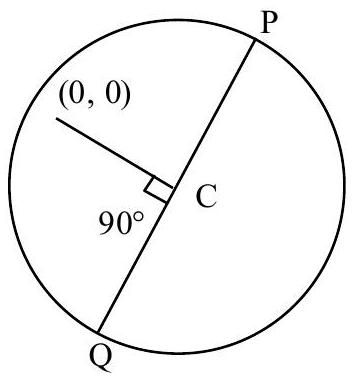
\includegraphics[max width=\textwidth, center]{2025_10_03_ad9ac098ef72e20a69f1g-6}\\
\(\mathrm{a}_{1}^{2}+\mathrm{b}_{1}^{2}+\mathrm{a}_{2}^{2}+\mathrm{b}_{2}^{2}=\mathrm{OP}^{2}+\mathrm{OQ}^{2}\)\\
\(=2(5+7)=24\)\\
84. The \(8^{\text {th }}\) common term of the series\\
\(\mathrm{S}_{1}=3+7+11+15+19+\ldots \ldots\),\\
\(\mathrm{S}_{2}=1+6+11+16+21+\ldots\).\\
is \(\_\_\_\_\) .

Official Ans. by NTA (151)\\
Allen Ans. (151)\\
Sol. \(\quad \mathrm{T}_{8}=11+(8-1) \times 20\)\\
\(=11+140=151\)\\
85. Let a line \(L\) pass through the point \(P(2,3,1)\) and be parallel to the line \(\mathrm{x}+3 \mathrm{y}-2 \mathrm{z}-2=0=\mathrm{x}-\mathrm{y}+2 \mathrm{z}\). If the distance of L from the point \((5,3,8)\) is \(\alpha\), then \(3 \alpha^{2}\) is equal to \(\_\_\_\_\) .

Official Ans. by NTA (158)\\
Allen Ans. (158)\\
Sol. \(\left|\begin{array}{ccc}\hat{i} & \hat{j} & \hat{k} \\ 1 & 3 & -2 \\ 1 & -1 & 2\end{array}\right|=4 \hat{i}-4 \hat{j}-4 \hat{k}\)\\
\(\therefore\) Equation of line is \(\frac{\mathrm{x}-2}{1}=\frac{\mathrm{y}-3}{-1}=\frac{\mathrm{z}-1}{-1}\)\\
Let Q be \((5,3,8)\) and foot of \(\perp\) from Q on this line be R .

Now, \(\mathrm{R} \equiv(\mathrm{k}+2,-\mathrm{k}+3,-\mathrm{k}+1)\)\\
DR of QR are ( \(\mathrm{k}-3,-\mathrm{k},-\mathrm{k}-7\) )\\
\(\therefore(1)(\mathrm{k}-3)+(-1)(-\mathrm{k})+(-1)(-\mathrm{k}-7)=0\)\\
\(\Rightarrow \mathrm{k}=-\frac{4}{3}\)\\
\(\therefore \alpha^{2}=\left(\frac{13}{3}\right)^{2}+\left(\frac{4}{3}\right)^{2}+\left(\frac{17}{3}\right)^{2}=\frac{474}{9}\)\\
\(\therefore 3 \alpha^{2}=158\)\\
86. If \(\int \sqrt{\sec 2 \mathrm{x}-1} \mathrm{dx}=\alpha \log _{\mathrm{e}}\left|\cos 2 \mathrm{x}+\beta+\sqrt{\cos 2 \mathrm{x}\left(1+\cos \frac{1}{\beta} \mathrm{x}\right)}\right|\) + constant, then \(\beta-\alpha\) is equal to \(\_\_\_\_\) .

Official Ans. by NTA (1)\\
Allen Ans. (1)

Sol. \(\quad \int \sqrt{\sec 2 \mathrm{x}-1} \mathrm{dx}=\int \sqrt{\frac{1-\cos 2 \mathrm{x}}{\cos 2 \mathrm{x}}} \mathrm{dx}\)\\
\(=\sqrt{2} \int \frac{\sin \mathrm{x}}{\sqrt{2 \cos ^{2} \mathrm{x}-1}} \mathrm{dx}\)\\
put \(\cos \mathrm{x}=\mathrm{t} \quad \Rightarrow-\sin \mathrm{xdx}=\mathrm{dt}\)\\
\(=-\sqrt{2} \int \frac{\mathrm{dt}}{\sqrt{2 \mathrm{t}^{2}-1}}\)\\
\(=-\ln |\sqrt{2} \cos x+\sqrt{\cos 2 x}|+c\)\\
\(=-\frac{1}{2} \ln \left|2 \cos ^{2} x+\cos 2 x+2 \sqrt{\cos 2 x} \cdot \sqrt{2} \cos x\right|+c\)\\
\(=-\frac{1}{2} \ln \left|\cos 2 x+\frac{1}{2}+\sqrt{\cos 2 x} \cdot \sqrt{1+\cos 2 x}\right|+c\)\\
\(\because \beta=\frac{1}{2}, \alpha=-\frac{1}{2} \Rightarrow \beta-\alpha=1\)\\
87. If the value of real number \(\mathrm{a}>0\) for which \(\mathrm{x}^{2}-5 \mathrm{ax} +1=0\) and \(x^{2}-a x-5=0\) have a common real roots is \(\frac{3}{\sqrt{2 \beta}}\) then \(\beta\) is equal to \(\_\_\_\_\) .

Official Ans. by NTA (13)\\
Allen Ans. (13)\\
Sol. Two equations have common root\\
\(\therefore(4 a)(26 a)=(-6)^{2}=36\)\\
\(\Rightarrow \mathrm{a}^{2}=\frac{9}{26} \quad \therefore \mathrm{a}=\frac{3}{\sqrt{26}} \Rightarrow \beta=13\)\\
88. The number of seven digits odd numbers, that can be formed using all the seven digits \(1,2,2,2,3,3,5\) is \(\_\_\_\_\) .\\
Official Ans. by NTA (240)\\
Allen Ans. (240)\\
Sol. Digits are \(1,2,2,2,3,3,5\)\\
If unit digit 5 , then total numbers \(=\frac{6!}{3!2!}\)\\
If unit digit 3 , then total numbers \(=\frac{6!}{3!}\)\\
If unit digit 1 , then total numbers \(=\frac{6!}{3!2!}\)\\
\(\therefore\) total numbers \(=60+60+120=240\)\\
89. A bag contains six balls of different colours. Two balls are drawn in succession with replacement. The probability that both the balls are of the same colour is p. Next four balls are drawn in succession with replacement and the probability that exactly three balls are of the same colours is \(q\). If \(p: q=m : n\), where \(m\) and \(n\) are coprime, then \(m+n\) is equal to \(\_\_\_\_\) .

Official Ans. by NTA (14)\\
Allen Ans. (14)\\
Sol. \(\mathrm{p}=\frac{{ }^{6} \mathrm{C}_{1}}{6 \times 6}=\frac{1}{6}\)\\
\(\mathrm{q}=\frac{{ }^{6} \mathrm{C}_{1} \times{ }^{5} \mathrm{C}_{1} \times 4}{6 \times 6 \times 6 \times 6}=\frac{5}{54}\)\\
\(\therefore \mathrm{p}: \mathrm{q}=9: 5 \Rightarrow \mathrm{~m}+\mathrm{n}=14\)\\
90. Let A be the area of the region\\
\(\left\{(x, y): y \geq x^{2}, y \geq(1-x)^{2}, y \leq 2 x(1-x)\right\}\).\\
Then 540 A is equal to\\
Official Ans. by NTA (25)\\
Allen Ans. (25)\\
Sol.\\
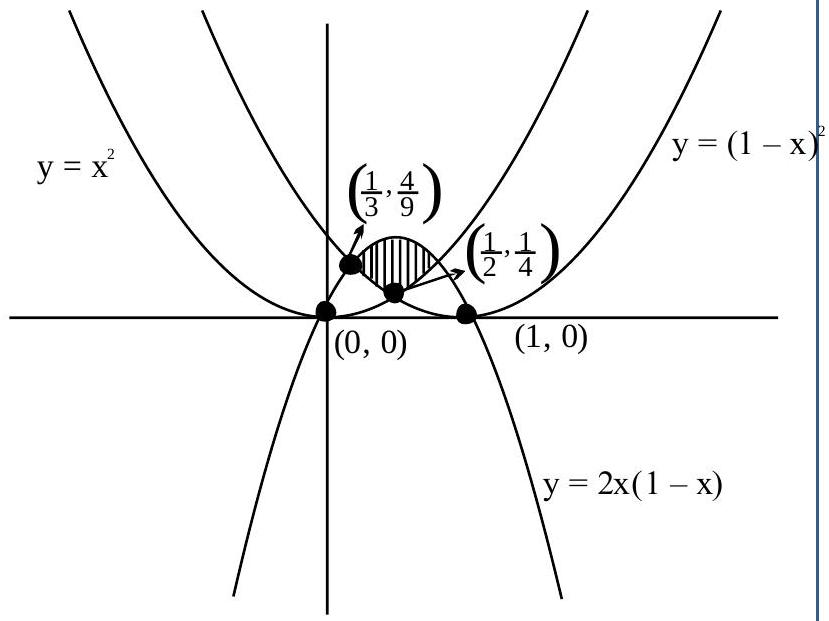
\includegraphics[max width=\textwidth, center]{2025_10_03_ad9ac098ef72e20a69f1g-8}\\
\(A=2 \int_{\frac{1}{3}}^{\frac{1}{2}}\left(2 x-2 x^{2}-(1-x)^{2}\right) d x\)\\
\(=2\left[2 \mathrm{x}^{2}-\mathrm{x}^{3}-\mathrm{x}\right]_{1 / 3}^{1 / 2}\)\\
\(\therefore \mathrm{A}=\frac{5}{108} \Rightarrow 540 \mathrm{~A}=\frac{5}{108} \times 540=25\)


\end{document}